% ============================================================
%  Failure-Mode-Specific Consensus for Multi-Agent LLM Ensembles
%  ACL/EMNLP-style conference paper draft.
%  Build: pdflatex main_acl && bibtex main_acl && pdflatex main_acl && pdflatex main_acl
% ============================================================
\documentclass[11pt]{article}

% --- Fonts ---
\usepackage[T1]{fontenc}
\usepackage[utf8]{inputenc}
% Use [review] for anonymous line-numbered submission mode.
\usepackage[final]{acl}

% --- Math ---
\usepackage{amsmath}
\usepackage{amssymb}
\usepackage{bm}

% --- Tables ---
\usepackage{booktabs}
\usepackage{multirow}
\usepackage{array}
\usepackage{tabularx}

% --- Figures ---
\usepackage{graphicx}
\usepackage{float}
\usepackage{placeins}

% --- Code ---
\usepackage{listings}
\lstset{
  basicstyle=\scriptsize\ttfamily,
  breaklines=true,
  breakatwhitespace=false,
  columns=fullflexible,
  frame=tb,
  numbers=none,
  keepspaces=true,
}

% --- Typography ---
\usepackage{microtype}

% --- Miscellaneous ---
\definecolor{darkblue}{rgb}{0,0,0.45}
\usepackage{enumitem}
\usepackage{url}

% Prefer regenerated conference figures; fall back to project-root assets.
\graphicspath{{figures_acl/}{../../}}

\setlength{\textfloatsep}{8pt plus 2pt minus 2pt}
\setlength{\floatsep}{8pt plus 2pt minus 2pt}
\setlength{\intextsep}{8pt plus 2pt minus 2pt}
\setlength{\dbltextfloatsep}{6pt plus 2pt minus 2pt}
\setlength{\dblfloatsep}{6pt plus 2pt minus 2pt}

% ============================================================
\title{\textbf{Failure-Mode-Specific Consensus\\
       for Multi-Agent LLM Ensembles}}
\author{Julia Novick}
\date{}
% ============================================================

\begin{document}
\maketitle

% ============================================================
\begin{abstract}
Multi-agent LLM ensembles often aggregate independent completions with
self-consistency, a majority vote over extracted answers. We study two failure
modes of this procedure and argue that they require different defenses rather
than a single universally optimal consensus rule. Invalid-format
outputs, such as empty or off-task generations, can contaminate voting when
answer extraction falls back to raw text. Coordinated valid-format wrong answers
create a separate problem: a small group of syntactically valid wrong answers can
form a concentrated semantic cluster that majority vote and confidence filtering
do not remove. We evaluate three mechanisms: abstention when no parseable final
answer is found (strict extraction), rather than treating malformed output as a
vote; a sliding-window token-probability filter (TopKMass); and an
embedding-space geometric median selector.

Across experiments on LLaMA 3.1 8B and Qwen2.5 7B using 100 cached questions
from GSM8K and StrategyQA with an 80-question held-out evaluation split per
model, strict answer extraction (a methodological correction to baseline
self-consistency that abstains rather than counting unparseable outputs as
votes) removes a 16.5 percentage point accuracy collapse in LLaMA majority-vote
results at high fault fractions. At $\beta=45\%$, the all-fault aggregate
favors TopKMass filtering plus strict majority vote over the strict-extraction
baseline (LLaMA 0.727 vs.\ 0.708; Qwen 0.656 vs.\ 0.648). TopKMass is the strongest of three tested
logprob-based correctness signals (LLaMA AUC/AP 0.612/0.810; Qwen 0.635/0.776),
although its absolute discriminative power is modest. Under coordinated synthetic
wrong-answer injection, geometric median nearest-centroid improves LLaMA
accuracy over strict majority vote by 7.5 percentage points (70.0\% vs.\ 62.5\%),
and a separate geometric analysis confirms that the geometric median remains
closer to the honest agents' outputs than the arithmetic mean across all tested
attack conditions. Multi-provider experiments delimit the scope of this defense:
geometric median helps when wrong answers form a tight coordinated cluster, but
not under natural provider diversity or scattered provider errors.
\end{abstract}

% ============================================================
\section{Introduction}
\label{sec:intro}

Multi-agent LLM ensembles improve output reliability by sampling multiple
independent completions and aggregating their answers. The most common
aggregation rule is self-consistency \citep{wang2023self}: extract a final answer
from each completion and return the plurality answer. This rule is simple and
effective when errors are independent and answer extraction is reliable, but it
offers little guidance for malformed outputs, confidence signals, or coordinated
wrong answers.

We study these issues through a failure-mode-specific lens. Self-consistency can
fail for qualitatively different reasons, and defenses that help in one regime
can be neutral or harmful in another.

\paragraph{Failure Mode 1: invalid-format outputs.}
Some completions contain no parseable final answer. If extraction falls back to
treating the entire output as a vote key, these malformed strings can contaminate
the vote pool. Strict answer extraction addresses this by abstaining when no
valid answer is found. TopKMass filtering provides a complementary mechanism by
identifying crash-like or off-task outputs whose token-probability traces fall
far outside the clean-agent distribution.

\paragraph{Failure Mode 2: coordinated valid-format wrong answers.}
A separate problem arises when a minority of agents produce extractable answers
that agree on the same wrong value. Strict extraction keeps these answers, and
confidence filtering does not remove them when their confidence traces are
spoofed or otherwise high. In this regime, the relevant structure is semantic:
if honest outputs form the dominant cluster in embedding space, geometric median
nearest-centroid aggregation can resist a smaller wrong-answer cluster.

Table~\ref{tab:intro-taxonomy} summarizes the taxonomy used throughout the paper.

\begin{table}[t]
\centering
\caption{Failure mode taxonomy. Each row maps one failure type to the mechanism
  that addresses it and its primary empirical role in this paper.}
\label{tab:intro-taxonomy}
\scriptsize
\begin{tabularx}{\columnwidth}{p{0.28\columnwidth}p{0.25\columnwidth}X}
\toprule
\textbf{Failure mode} & \textbf{Mechanism that helps} & \textbf{Main empirical role} \\
\midrule
Invalid or unparseable outputs
  & Strict answer extraction
  & Prevents raw malformed text from entering the vote \\[4pt]
Low-confidence crash or drift outputs
  & TopKMass filtering
  & Removes agents outside the clean confidence distribution \\[4pt]
Coordinated valid wrong answers
  & Geometric median nearest-centroid
  & Selects from the semantic center of the admitted pool \\[4pt]
Scattered provider errors
  & Majority vote
  & Remains competitive when wrong answers do not form a cluster \\
\bottomrule
\end{tabularx}
\end{table}

This paper makes four contributions:
\begin{enumerate}[leftmargin=*, itemsep=2pt]
  \item A failure-mode taxonomy for multi-agent LLM consensus, separating
        invalid-format failures from coordinated valid-format wrong answers.
  \item An evaluation of TopKMass filtering with the same stable-region statistic
        used for both calibration and signal-quality analysis.
  \item An embedding-space geometric median selector and centroid-shift analysis
        for coordinated synthetic wrong-answer injection.
  \item A set of ablations across two open-weight models, two datasets, multiple
        fault types, and multi-provider settings that identifies where each
        mechanism helps and where it does not.
\end{enumerate}

% ============================================================
\section{Related Work}
\label{sec:related}

\paragraph{Self-consistency \citep{wang2023self}}
is the standard approach to multi-sample LLM aggregation: sample $N$
chain-of-thought completions, extract the final answer token from each, and
return the plurality answer. Our work takes self-consistency as the primary
baseline, identifies its failure modes under fault injection and coordinated
attack, and proposes complementary mechanisms to address each failure mode.
Strict extraction (abstaining when no parseable answer is found) is also a
methodological improvement applicable to any self-consistency implementation.

\paragraph{DecentLLMs \citep{jo2024decentllms}}
is the closest prior system-level approach. DecentLLMs uses a worker/evaluator
structure where each candidate output is scored by multiple evaluators across
several criteria, and the geometric median is applied over the resulting score
matrix to select a winner. The key difference is the aggregation space:
DecentLLMs applies geometric median in criterion score space (evaluator ratings),
while our system applies geometric median in sentence embedding space (output
text semantics). The two approaches address different failure modes; the
published DecentLLMs method does not use per-token logprobs for
confidence-based pre-filtering.

\paragraph{Byzantine Fault Tolerance \citep{lamport1982byzantine,castro1999practical}}
provides the analytical scaffolding for our liveness threshold and fault model.
Classical BFT protocols achieve Byzantine-fault tolerance with $N \geq 3f+1$
nodes through multi-round message passing with $O(N^2)$ message complexity. Our
system is not a BFT protocol: it is a one-shot aggregation pipeline with a
confidence filter, and the setting is a homogeneous single-model pool where
agents have no incentive to collude. The BFT framing motivates the liveness
threshold ($2f+1$ admitted agents required, $f = \lfloor(N-1)/3\rfloor$) and the
fault fraction regime ($\beta=0.45$ with $N=7$ injects $\lfloor7\times0.45\rfloor=3$ faults,
exceeding the tolerance of $f=2$, which causes consistent liveness fallback).

\paragraph{Geometric median robustness \citep{weiszfeld1937point,minsker2015geometric}}
provides the theoretical foundation for the embedding-space selector. The
geometric median minimizes sum of $\ell_2$ distances, whereas the arithmetic mean
minimizes sum of squared distances. In Euclidean space, the geometric median has
a breakdown point of $1/2$, so a minority of outlying points cannot move it
arbitrarily far. Our centroid-shift analysis is consistent with this mechanism,
but we treat it as mechanistic evidence rather than a sufficient condition for
accuracy improvement.

\paragraph{Minimum Bayes Risk (MBR) decoding \citep{eikema2020map}}
selects the hypothesis that minimizes expected loss across a candidate pool using
pairwise similarity. Our geometric median nearest-centroid is conceptually
related but operates in embedding space and has $O(N)$ complexity after
embedding, compared to $O(N^2)$ pairwise evaluation for MBR.

\paragraph{Sentence embedding aggregation \citep{li2023making}}
applies embedding clustering for reasoning answer selection. Our approach uses
geometric median rather than $k$-means or nearest-neighbor clustering, providing
a different robustness objective for clustered outliers.

\paragraph{Calibration and per-token confidence \citep{guo2017calibration}}
motivate Module~1's signal design. TopKMass is a sliding-window
stability measure (the mean sum of top-5 token probabilities over a $W=64$
window) rather than an instantaneous per-token confidence. This design measures
whether a model maintains high-confidence generation across a sequence and is
the confidence signal evaluated in our experiments.

% ============================================================
\section{System Description}
\label{sec:system}

\subsection{Architecture}
\label{sec:arch}

The pipeline separates GPU-intensive generation from CPU evaluation. Phase~1
(offline generation) uses \texttt{vLLM} with temperature$=0.7$ and logprobs$=5$
to produce $N=7$ completions per question, caching all outputs and per-token
top-5 logprobs to a JSON file. Phase~2 (evaluation) runs entirely on cached
data with no GPU or \texttt{vLLM} dependency.

All data passed between modules conforms to two typed dataclasses:

\begin{table}[t]
\centering
\caption{Data contracts between pipeline modules.}
\label{tab:data-contracts}
\scriptsize
\begin{tabularx}{\columnwidth}{lX}
\toprule
\textbf{Object} & \textbf{Fields} \\
\midrule
\texttt{AgentGeneration}
  & \texttt{agent\_id}, \texttt{output\_text}, \texttt{token\_logprobs}
    (flat list, length $5T$), \texttt{is\_faulty}, \texttt{fault\_type},
    optional \texttt{model\_id}, optional \texttt{provider} \\
\texttt{ConsensusResult}
  & \texttt{final\_answer}, \texttt{admitted\_agents}, \texttt{is\_low\_confidence} \\
\bottomrule
\end{tabularx}
\end{table}

\subsection{Module 1: TopKMass Confidence Filter}
\label{sec:module1}

\paragraph{Signal computation.}
For each agent with $T$ output tokens, the token logprob list has length $5T$
(top-5 logprobs per position). The TopKMass trajectory is computed using a
causal sliding window of width $W=64$:

\begin{equation}
\begin{aligned}
\mathrm{TopKMass}(t)
  &= \frac{1}{\min(t+1,\,W)}
     \sum_{i=s(t)}^{t} m_i, \\
s(t) &= \max(0,\,t-W+1), \\
m_i &= \sum_{k=1}^{5} \exp(\mathrm{logprob}_{i,k}).
\end{aligned}
\label{eq:topkmass}
\end{equation}

This is implemented in $O(T)$ via prefix sums (\texttt{numpy.cumsum}), avoiding
an $O(T \times W)$ inner loop.

The scalar score for each agent is derived in three steps:
\begin{enumerate}[leftmargin=*, itemsep=2pt]
  \item \textbf{Trajectory:} at each token position, sum the top-5 token
        probabilities using the $W=64$ causal sliding window, producing one
        value per token position.
  \item \textbf{Post-warmup:} skip the first $W$ positions so the scalar score
        is computed from the same steady-state portion of each trajectory. The
        stable portion starts at position $W=64$.
  \item \textbf{Mean:} average the stable-region values into a single scalar
        per agent.
\end{enumerate}

\paragraph{Warmup normalization.}
For outputs shorter than $2W$ tokens (common in StrategyQA with
\texttt{max\_tokens}$=128$), a large fraction of the trajectory lies in the
initial region before a full-window steady state is available. We therefore use
the post-warmup slice as the canonical per-agent statistic so short and long
outputs are scored from the same portion of the trajectory. The stable-region
mean is computed on positions $[W{:}]$, falling back to the full trajectory when
output length is at most $W$. This same statistic is used in filtering and
$\tau$ calibration.

\paragraph{Threshold calibration.}
$\tau$ is calibrated at the 5th percentile of stable-region TopKMass scores on
a 20\% shuffled dev slice. Shuffling is critical: the cache orders GSM8K
questions first (indices 0--49), and without shuffling the dev slice draws
entirely from higher-confidence GSM8K questions, biasing $\tau$ upward and
causing approximately 50\% liveness fallback at $\beta=0$. With shuffling (fixed
seed$=42$), the 5th-percentile $\tau$ is calibrated on a representative mix and
produces approximately 5\% clean-agent false rejection.

\paragraph{Liveness fallback.}
The tolerated fault count is $f = \lfloor(N-1)/3\rfloor$ ($N=7$ gives $f=2$;
$N=5$ gives $f=1$). If fewer than $2f+1$ agents pass filtering, all available
agents are admitted and the result is flagged as low-confidence. This ensures the
pipeline always produces an answer.

Table~\ref{tab:fault-scores} summarizes expected behavior by injected fault type.

\begin{table*}[!t]
\centering
\caption{TopKMass score and Module~1 outcome by fault type.}
\label{tab:fault-scores}
{\footnotesize
\setlength{\tabcolsep}{5pt}
\renewcommand{\arraystretch}{1.08}
\begin{tabularx}{\textwidth}{p{0.16\textwidth}p{0.32\textwidth}X}
\toprule
\textbf{Fault} & \textbf{TopKMass Score} & \textbf{Module 1 Outcome} \\
\midrule
F1 (crash)
  & 0.0 (empty logprobs)
  & Dropped unconditionally \\
F3 (drifter)
  & ${\approx}2.3{\times}10^{-4}$ (logprob spoof: $-10.0$ per entry)
  & Dropped (below any $\tau > 0.001$) \\
F2 (Experiment~1 invalid-format injection)
  & 1.00 (logprob spoof: sum $= 1.00$ exactly)
  & \textbf{Passes} at any $\tau \leq 1.0$ \\
Clean agent
  & $[0.91,\,1.00]$ LLaMA, $[0.97,\,1.00]$ Qwen (5th percentile to max over clean agents)
  & Passes unless rare outlier \\
\bottomrule
\end{tabularx}
}
\end{table*}

Experiment~1 F2 logprobs are spoofed to TopKMass$=1.00$ because the construction
$[\log(0.95),\log(0.02),\log(0.015),\log(0.010),\log(0.005)]$ gives top-5
probabilities summing to exactly 1.00 per token position. This is the
mathematical maximum of TopKMass and guarantees Byzantine agents pass Module~1
at any $\tau \leq 1.00$, regardless of $\tau$ calibration.

\subsection{Module 2: Geometric Median Nearest-Centroid}
\label{sec:module2}

Admitted agents' output texts are embedded using
\texttt{sentence-transformers/all-mpnet-base-v2} (768-dimensional). The
geometric median of the embedding matrix is computed by minimizing:

\begin{equation}
f(\mathbf{y}) = \sum_{i=1}^{N} \|\mathbf{x}_i - \mathbf{y}\|_2
\label{eq:geomed}
\end{equation}

via L-BFGS-B with analytic gradient:

\begin{equation}
\nabla f(\mathbf{y}) = -\sum_{i=1}^{N}
  \frac{\mathbf{x}_i - \mathbf{y}}{\|\mathbf{x}_i - \mathbf{y}\|_2}
\label{eq:geomed-grad}
\end{equation}

and denominator clamping at $10^{-10}$. The final answer is the
\texttt{output\_text} of the agent with minimum Euclidean distance to this
geometric median (nearest-centroid selection). The reported homogeneous
experiments use this nearest-centroid selector for the primary pipeline
condition, named \texttt{full\_system} in Experiment~1 and \texttt{stage1\_only}
in Experiment~3. Implementation provenance is provided in Appendix~\ref{app:code}.

Earlier aggregation variants included bidirectional natural language inference
(NLI) entailment verification and distance-weighted answer voting, in which each
agent's extracted answer is weighted by its proximity to the embedding-space
geometric median before plurality voting. These are retained only as ablations
and are not the recommended geometric-median condition.

\subsection{Ablation Conditions}
\label{sec:conditions}

Experiment~1 reports the homogeneous ablations below. Experiment~3 reuses the
nearest-centroid method as \texttt{stage1\_only} and reports
\texttt{full\_pipeline} only for the distance-weighted voting ablation.

\begin{table*}[!t]
\centering
\caption{Pipeline conditions used in Experiment~1 and Experiment~3.}
\label{tab:conditions}
{\footnotesize
\setlength{\tabcolsep}{5pt}
\renewcommand{\arraystretch}{1.08}
\begin{tabularx}{\textwidth}{p{0.25\textwidth}p{0.32\textwidth}X}
\toprule
\textbf{Condition} & \textbf{TopKMass role} & \textbf{Aggregation} \\
\midrule
\texttt{baseline}
  & None
  & Strict majority vote with abstention on unparseable outputs \\[4pt]
\texttt{soft\_weighting}
  & Aggregation weights (no admission threshold)
  & TopKMass-weighted geometric median \\[4pt]
\texttt{hard\_only}
  & Hard admission filter + liveness fallback
  & Strict majority vote \\[4pt]
\texttt{full\_system} / \texttt{stage1\_only}
  & Hard admission filter + liveness fallback
  & Geometric median nearest-centroid \\
\bottomrule
\end{tabularx}
}
\end{table*}

\subsection{Fault Injection}
\label{sec:faults}

The fault injector (\texttt{faults/injector.py}) applies deterministic mutations
to cached data. Exactly $\lfloor N \times \beta \rfloor$ agents are mutated per
question, selected via \texttt{random.Random(seed).sample}. F1 agents receive
empty \texttt{output\_text} and \texttt{token\_logprobs}. In Experiment~1, F2
agents receive a fixed unparseable wrong-answer template and logprobs spoofed to
TopKMass$=1.00$; this construction is distinct from the valid-format
coordinated wrong-answer injection studied in Experiment~3. F3 agents receive
syntactically plausible off-task text and token logprobs set
uniformly to $-10.0$, producing a TopKMass score of approximately
$2.3\times10^{-4}$ and reliably triggering filter rejection. The \texttt{mix}
condition assigns each mutated agent an independently drawn fault type. Original
\texttt{AgentGeneration} objects are never mutated; clean agents are returned by
reference.

% ============================================================
\section{Experiment 1: Fault Injection Ablation}
\label{sec:exp1}

\subsection{Setup}
\label{sec:exp1-setup}

We evaluate four pipeline conditions across $N \in \{5,7\}$ agents,
$\beta \in \{0,\,0.15,\,0.30,\,0.45\}$ fault fraction, and fault types
\{F1, F2, F3, mix\} on 100 cached questions (50 GSM8K multi-step arithmetic,
50 StrategyQA commonsense yes/no). LLaMA 3.1 8B Instruct \citep{metaai2024llama} and Qwen2.5 7B
Instruct \citep{qwenteam2024qwen25} each receive their own cached generation sets ($N=7$ agents,
temperature$=0.7$, \texttt{max\_tokens}$=512$ for GSM8K and 128 for
StrategyQA). $\tau$ is auto-calibrated per run on a 20\% dev split; all reported
accuracies use the remaining 80 evaluation questions per model.

Strict answer extraction is applied to \texttt{baseline} and \texttt{hard\_only}:
agents whose output contains no parseable answer return \texttt{None} and are
excluded from the vote. Earlier runs without strict extraction showed a 16.5
percentage point LLaMA accuracy collapse at $\beta=0.45$, which strict extraction
corrects.

\subsection{Results}
\label{sec:exp1-results}

\begin{table*}[!t]
\centering
\caption{Experiment~1 accuracy by condition, model, and fault fraction
  (averaged over $N \in \{5,7\}$ and all fault types).}
\label{tab:exp1-results}
\footnotesize
\setlength{\tabcolsep}{4.2pt}
\begin{tabularx}{\textwidth}{l X ccccc}
\toprule
\textbf{Model} & \textbf{Condition} & \textbf{N=1 (ref)} & $\bm{\beta}=0$\%
  & $\bm{\beta}=15$\% & $\bm{\beta}=30$\%
  & $\bm{\beta}=45$\% \\
\midrule
\multirow{4}{*}{LLaMA}
  & \texttt{baseline} (self-consistency) & 0.713 & 0.756 & 0.769 & 0.736 & 0.708 \\
  & \texttt{soft\_weighting}             & 0.713 & 0.713 & 0.725 & 0.727 & 0.688 \\
  & \texttt{hard\_only}                  & 0.713 & 0.750 & 0.763 & 0.745 & \textbf{0.727} \\
  & \texttt{full\_system} (\texttt{stage1\_only}) & 0.713 & 0.700 & 0.723 & 0.733 & 0.653 \\
\midrule
\multirow{4}{*}{Qwen}
  & \texttt{baseline} (self-consistency) & 0.675 & 0.669 & 0.663 & 0.672 & 0.648 \\
  & \texttt{soft\_weighting}             & 0.675 & 0.650 & 0.650 & 0.644 & 0.663 \\
  & \texttt{hard\_only}                  & 0.675 & 0.669 & 0.663 & 0.675 & \textbf{0.656} \\
  & \texttt{full\_system} (\texttt{stage1\_only}) & 0.675 & 0.650 & 0.650 & 0.644 & 0.645 \\
\bottomrule
\end{tabularx}
\end{table*}

The $N=1$ single-agent reference is immune to fault injection
($\lfloor 1 \times \beta \rfloor = 0$ for any $\beta < 1.0$) and serves as the
no-consensus anchor. LLaMA $N=1$ accuracy (0.713) is consistent with published
greedy-decoding results of approximately 73\% \citep{metaai2024llama}; the
mixed-benchmark setting (50\% StrategyQA) accounts for the slight downward shift
from GSM8K-only benchmarks.

\subsection{Key Findings}
\label{sec:exp1-findings}

\paragraph{Finding 1: Strict extraction is the primary Experiment 1 result.}
Without strict extraction, the LLaMA baseline at $\beta=0.45$ was 0.543; with
strict extraction it is 0.708, a 16.5pp improvement. The gap arose because the
Experiment~1 F2 template and F3 agents have unscorable outputs that contributed
their full text as vote keys. These keys could win plurality when
parseable-answer agents did not form a single
dominant extracted answer. Strict extraction removes these spurious votes. The
4.1pp Qwen improvement (0.607 to 0.648) is smaller because Qwen's individual
answer-extraction accuracy is higher, leaving fewer invalid votes. This isolates
answer extraction as an important confound in self-consistency evaluation.

\paragraph{Finding 2: \texttt{hard\_only} is strongest in the all-fault aggregate
at high fault load.}
At $\beta=0.45$, \texttt{hard\_only} outperforms \texttt{baseline} by 1.9pp for
LLaMA (0.727 vs.\ 0.708) and by 0.8pp for Qwen (0.656 vs.\ 0.648). These small
differences should be interpreted cautiously, but they are consistent with the
intended mechanism: TopKMass filtering drops F1 and F3 agents before strict
majority voting. The invalid-format-only slices are less uniform, as the
high-drifter cell in Finding~3 shows.

\paragraph{Finding 3: \texttt{soft\_weighting} is strongest in the high-drifter
cell.}
At $N=7$, $\beta=0.45$, F3-only, LLaMA \texttt{soft\_weighting} achieves 0.725
vs.\ 0.638 for \texttt{baseline}. At high drifter fractions, Module~1
hard-filters all F3 agents, triggering liveness fallback at 100\% of questions
and reverting to the full pool. Soft-weighting avoids this by continuously
down-weighting low-confidence agents rather than hard-filtering them.

\paragraph{Finding 4: \texttt{full\_system} underperforms for invalid-format
faults.}
At $\beta=0.45$, \texttt{full\_system} is 7.4pp below \texttt{hard\_only} for
LLaMA (0.653 vs.\ 0.727). When the liveness fallback triggers and admits the
full pool (including drifter or crash agents), geometric median in embedding
space can be drawn toward outlier embeddings even while strict majority vote
correctly ignores agents with no parseable answer. The advantage of
\texttt{full\_system} emerges in Experiment~3, where the threat structure is
different.

\paragraph{Finding 5: Qwen $\beta=0$ fallback rate is elevated.}
At $\beta=0$, \texttt{hard\_only} and \texttt{full\_system} trigger liveness
fallback on 13.75\% of Qwen questions (vs.\ 5.0\% for LLaMA). Although Qwen's
overall clean TopKMass scores are higher, its 5th-percentile threshold still
removes enough clean agents in some rounds to trigger more liveness fallbacks.
Accuracy recovers via liveness fallback, but this calibration artifact reduces
the filter's net contribution. Adaptive
per-model $\tau$ calibration with larger dev slices could reduce this fallback
rate.

See Figure~\ref{fig:accuracy-beta} for accuracy vs.\ $\beta$ line charts and
Figure~\ref{fig:fault-breakdown} for per-fault-type breakdown at $\beta=0.45$.

\begin{figure*}[t]
\centering
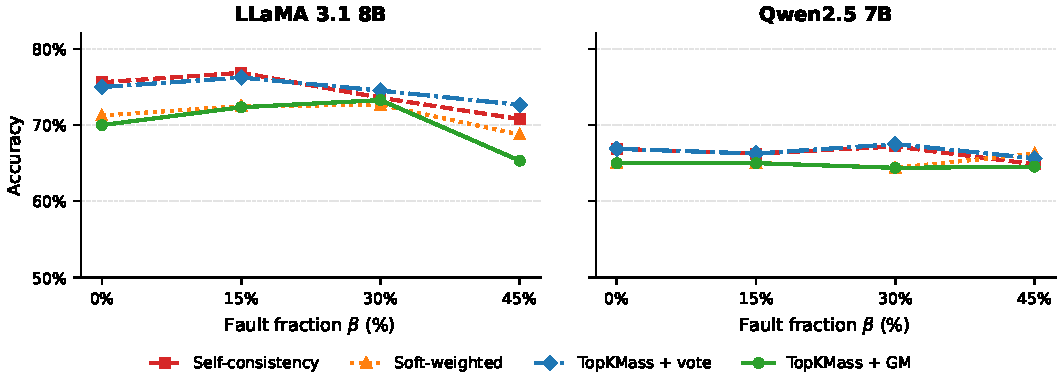
\includegraphics[width=\linewidth]{accuracy_vs_beta_no_n1_acl}
\caption{Experiment~1: accuracy vs.\ fault fraction $\beta$ for each condition
  and model (N=1 reference excluded; see Figure~\ref{fig:accuracy-beta-n1} in
  Appendix~\ref{app:figures} for the version including the N=1 reference line).}
\label{fig:accuracy-beta}
\end{figure*}

\begin{figure*}[t]
\centering
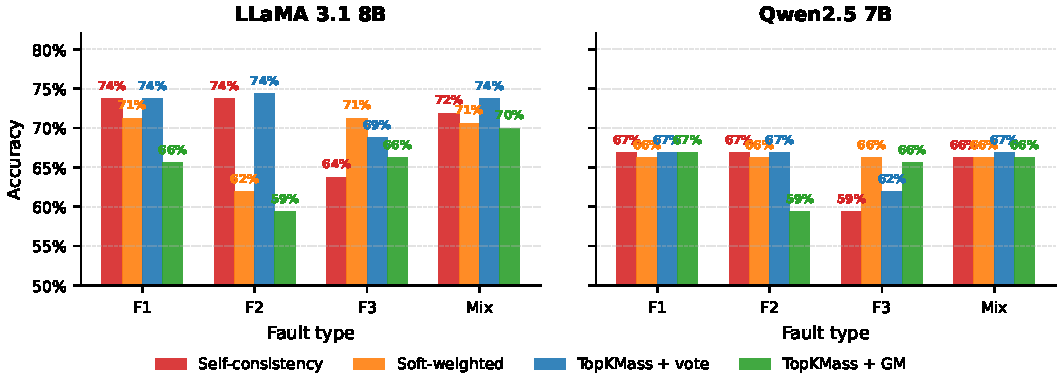
\includegraphics[width=\linewidth]{fault_type_breakdown_acl}
\caption{Experiment~1: per-fault-type accuracy breakdown at $\beta=0.45$ for
  both models. Bars show accuracy for each condition across F1, F2, F3, and mix
  fault types.}
\label{fig:fault-breakdown}
\end{figure*}

% ============================================================
\section{Experiment 2: TopKMass Signal Quality Validation}
\label{sec:exp2}

\subsection{Setup}
\label{sec:exp2-setup}

Experiment~2 evaluates TopKMass as a filter signal by measuring its predictive
value for individual agent correctness, compared to two simpler logprob-based
alternatives. All 700 agents per model (100 questions $\times$ 7 agents) are
labeled \texttt{is\_correct} via shared answer extraction against ground truth.
Three signals are computed from \texttt{token\_logprobs}:

\begin{itemize}[leftmargin=*, itemsep=2pt]
  \item \textbf{TopKMass (stable-region mean):} the post-warmup mean of the
        causal $W=64$ TopKMass trajectory, falling back to the full trajectory
        for outputs of length at most $W$. This is the same statistic used for
        filtering and $\tau$ calibration.
  \item \textbf{Negated mean token entropy:} $-\mathrm{mean}(-\sum p \log p)$
        over token positions, using top-5 unnormalized probabilities.
  \item \textbf{Negated logprob variance:} $-\mathrm{var}(\mathrm{mean~logprob~per~position})$,
        negated so higher is better (lower variance $=$ more stable confidence).
\end{itemize}

All signals are oriented so that higher values indicate greater confidence (more
likely correct). Receiver operating characteristic area under the curve
(ROC-AUC) and average precision (AP) are computed for each signal as a binary
correctness classifier.

\subsection{Results}
\label{sec:exp2-results}

\begin{table}[h]
\centering
\caption{Signal quality for correctness prediction (700 agents per model).
  Higher is better for all metrics.}
\label{tab:signal-quality}
{\scriptsize
\setlength{\tabcolsep}{4pt}
\renewcommand{\arraystretch}{1.04}
\begin{tabularx}{\columnwidth}{lXcc}
\toprule
\textbf{Model} & \textbf{Signal} & \textbf{AUC} & \textbf{AP} \\
\midrule
\multirow{3}{*}{LLaMA}
  & \textbf{TopKMass}        & \textbf{0.612} & \textbf{0.810} \\
  & Negated Entropy          & 0.580 & 0.791 \\
  & Negated Logprob Variance & 0.448 & 0.675 \\
\midrule
\multirow{3}{*}{Qwen}
  & \textbf{TopKMass}        & \textbf{0.635} & \textbf{0.776} \\
  & Negated Entropy          & 0.616 & 0.765 \\
  & Negated Logprob Variance & 0.538 & 0.678 \\
\bottomrule
\end{tabularx}
}
\end{table}

\subsection{Key Findings}
\label{sec:exp2-findings}

\paragraph{TopKMass is the strongest of the tested predictors on both models,}
achieving the highest AUC and AP on LLaMA (0.612, 0.810) and Qwen (0.635,
0.776). The absolute AUC values are modest, so this result should be interpreted
as comparative signal validation rather than strong correctness prediction.

\paragraph{Logprob variance performs below chance for LLaMA (AUC$=0.448$).}
High logprob variance reflects natural variation in token confidence across a
multi-step reasoning chain (for example, arithmetic steps alternating with
reasoning steps at different confidence levels), not output unreliability. Using
variance as a filter signal would disadvantage models on precisely the tasks
(multi-step reasoning) where they perform strongly. This negative result
supports the sliding-window design of TopKMass, which measures confidence
stability across the sequence rather than raw variance.

\paragraph{No signal is a correctness oracle.}
Both correct and incorrect agents cluster in a high-confidence range
(5th percentile to max: $[0.91,\,1.00]$ for LLaMA, $[0.97,\,1.00]$ for Qwen)
with heavy overlap; LLaMA has a small lower tail extending to a minimum of
approximately 0.72. The
correct-agent TopKMass median is higher than the incorrect-agent median (see
Figure~\ref{fig:topkmass-dist}, which shows the distribution for clean LLaMA
agents). TopKMass's primary value as a
filter is detecting agents far outside this clean cluster: F1 agents score
exactly 0.0 (empty logprobs), F3 drifter agents score ${\approx}2.3\times10^{-4}$
(logprob spoof: $-10.0$ per entry). These are detectable at any $\tau > 0.001$,
which explains why Module~1 can remove crash and drifter agents while retaining
most clean agents.



See Figure~\ref{fig:signals} for ROC curves, TopKMass scatter, and
Precision-Recall curves.

\begin{figure*}[t]
\centering
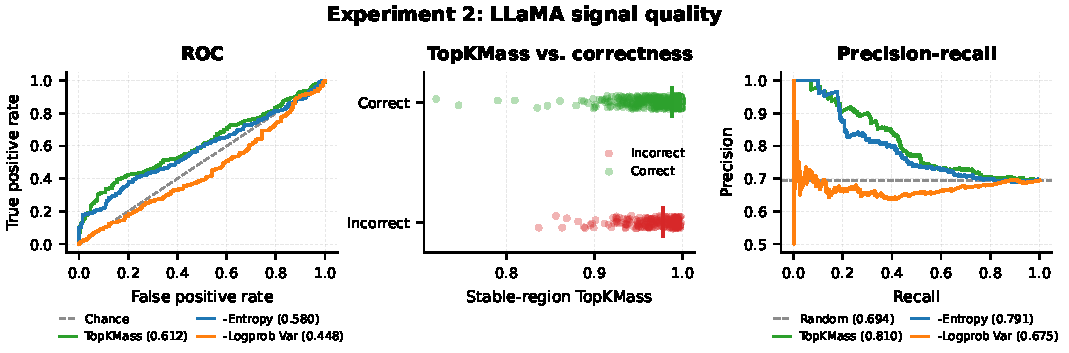
\includegraphics[width=\linewidth]{experiment_2_signals_llama_acl}
\caption{Experiment~2 (LLaMA 3.1 8B): signal quality panels. Panel~A: ROC
  curves for all three signals. Panel~B: TopKMass score vs.\ correctness
  (jittered scatter with class medians). Panel~C: Precision-Recall curves.}
\label{fig:signals}
\end{figure*}

% ============================================================
\section{Experiment 3: Coordinated Adversarial Attack}
\label{sec:exp3}

\subsection{Setup}
\label{sec:exp3-setup}

Experiment~3 evaluates coordinated synthetic wrong-answer injection: a minority
of agents produce valid extractable wrong answers, agree on the same wrong value,
and spoof logprobs to pass Module~1. The setting is $N=7$, $f=2$ (2 injected
agents, 5 clean agents). Three coordination degrees are evaluated:

\begin{itemize}[leftmargin=*, itemsep=2pt]
  \item \textbf{Uncoordinated:} The 2 Byzantine agents produce semantically
        different wrong texts. Both spoof TopKMass$=1.00$, so they pass
        Module~1, but they embed far apart in sentence space and cannot form a
        coherent adversarial cluster.
  \item \textbf{Coordinated:} Both agents produce the same wrong answer derived
        from the ground truth (``The answer is \{opposite\}.'' for StrategyQA;
        ``The answer is \{gt+7\}.'' for GSM8K). They cluster at a single point
        in embedding space.
  \item \textbf{Max-confidence coordinated:} Identical to coordinated in answer
        content, with a higher-confidence logprob spoof. Because both coordinated
        settings achieve TopKMass$=1.00$, this condition is numerically
        equivalent to coordinated for Module~1 admission and is reported as a
        duplicate stress setting rather than a stronger attack.
\end{itemize}

Three pipeline conditions are compared: strict answer majority vote,
geometric median nearest-centroid, and a distance-weighted voting ablation
(see Appendix~\ref{app:code} for implementation provenance).

\subsection{Centroid Shift Metric}
\label{sec:centroid-shift}

For each question, we compute the distance from the arithmetic mean and geometric
median of all 7 agents' embeddings to the honest-agent centroid (mean embedding
of the 5 clean agents):

\begin{equation}
\delta = d(\bar{\mathbf{x}},\,\boldsymbol{\mu}_h)
       - d(\mathbf{m},\,\boldsymbol{\mu}_h)
\label{eq:centroid-shift}
\end{equation}

where $\bar{\mathbf{x}}$ is the arithmetic mean embedding, $\mathbf{m}$ is the
geometric median, and $\boldsymbol{\mu}_h$ is the honest-agent centroid. Positive
$\delta$ indicates the geometric median stays closer to the honest cluster than
the arithmetic mean. This metric is computed before any filtering and averaged
across all evaluation questions.

\subsection{Results}
\label{sec:exp3-results}

\begin{table*}[t]
\centering
\caption{Experiment~3: accuracy by coordination degree and pipeline condition
  (80 evaluation questions per model). Best result per model per coordination
  degree is in bold.}
\label{tab:exp3-accuracy}
\small
\begin{tabular}{llcc}
\toprule
\textbf{Coordination} & \textbf{Condition}
  & \textbf{LLaMA Acc.} & \textbf{Qwen Acc.} \\
\midrule
\multirow{3}{*}{Uncoordinated}
  & \texttt{majority\_answer\_vote} & \textbf{72.5\%} & \textbf{65.0\%} \\
  & \texttt{stage1\_only}           & 67.5\%          & 63.75\%         \\
  & \texttt{full\_pipeline}         & 57.5\%          & 48.75\%         \\
\midrule
\multirow{3}{*}{Coordinated}
  & \texttt{majority\_answer\_vote} & 62.5\%          & \textbf{65.0\%} \\
  & \texttt{stage1\_only}           & \textbf{70.0\%} & \textbf{65.0\%} \\
  & \texttt{full\_pipeline}         & 56.25\%         & 48.75\%         \\
\midrule
\multirow{3}{*}{Max-conf.\ coord.}
  & \texttt{majority\_answer\_vote} & 62.5\%          & \textbf{65.0\%} \\
  & \texttt{stage1\_only}           & \textbf{70.0\%} & \textbf{65.0\%} \\
  & \texttt{full\_pipeline}         & 56.25\%         & 48.75\%         \\
\bottomrule
\end{tabular}
\end{table*}

\begin{table*}[t]
\centering
\caption{Centroid shift metric. \texttt{dist\_mean} and \texttt{dist\_gm}: distance
  from the arithmetic mean and geometric median to the honest cluster centroid
  (smaller $=$ closer to honest outputs). $\delta = \texttt{dist\_mean} - \texttt{dist\_gm}$:
  positive values indicate the geometric median remains closer to the honest
  cluster than the arithmetic mean.}
\label{tab:centroid-shift}
\small
\begin{tabular}{llccc}
\toprule
\textbf{Coordination} & \textbf{Model}
  & \textbf{dist\_mean} & \textbf{dist\_gm}
  & $\bm{\delta}$ (mean$-$gm) \\
\midrule
\multirow{2}{*}{Uncoordinated}
  & LLaMA & 0.339 & 0.095 & \textbf{$+$0.244} \\
  & Qwen  & 0.347 & 0.066 & \textbf{$+$0.282} \\
\midrule
\multirow{2}{*}{Coordinated}
  & LLaMA & 0.353 & 0.113 & \textbf{$+$0.239} \\
  & Qwen  & 0.366 & 0.076 & \textbf{$+$0.290} \\
\midrule
\multirow{2}{*}{Max-conf.\ coord.}
  & LLaMA & 0.353 & 0.113 & \textbf{$+$0.239} \\
  & Qwen  & 0.366 & 0.076 & \textbf{$+$0.290} \\
\bottomrule
\end{tabular}
\end{table*}

\subsection{Key Findings}
\label{sec:exp3-findings}

\paragraph{Finding 1: geometric median nearest-centroid improves LLaMA under
coordinated injection.}
Under uncoordinated conditions, majority vote outperforms geometric median
nearest-centroid (72.5\% vs.\ 67.5\%) because the two diverse wrong-answer
embeddings do not form a cluster. Under coordinated injection, the two injected
agents return the same wrong answer, reducing majority vote accuracy to 62.5\%.
Geometric median nearest-centroid reaches 70.0\%, a 7.5pp improvement over
majority vote in this setting.

\paragraph{Finding 2: the weighted-vote ablation is not retained.}
LLaMA weighted-vote accuracy ranges from 56.25\% to 57.5\% across coordination
degrees, and Qwen weighted-vote accuracy is 48.75\% across conditions. Its
failure mode is vote fragmentation: diverse correct answers can split weighted
vote mass, while a coordinated wrong-answer cluster concentrates weight on one
extractable answer. Geometric median nearest-centroid (70.0\% LLaMA, 65.0\%
Qwen under coordinated injection) is therefore the retained geometric-median
condition for this experiment.

\paragraph{Finding 3: Qwen Experiment~3 is neutral.}
Under coordinated injection, geometric median nearest-centroid and majority vote
both achieve 65.0\% accuracy for Qwen. The liveness fallback rate for geometric
median nearest-centroid is 11.25\% (vs.\ 2.5\% for LLaMA): Qwen's calibrated
threshold removes enough clean agents to trigger fallback on roughly 1 in 9
questions, reverting to the full 7-agent pool. The centroid shift deltas
remain positive ($+0.282$ to $+0.290$), but this mechanistic signal is not
sufficient to produce an accuracy gain for Qwen. Adaptive $\tau$ calibration
tuned to Qwen's score distribution (Section~\ref{sec:conclusion}, future
direction~2) could reduce this fallback rate and potentially recover the accuracy
gain seen for LLaMA.

\paragraph{Finding 4: centroid shift supports the mechanism but does not imply
accuracy gains.}
Positive $\delta$ is observed in all 6 conditions. Coordination increases
\texttt{dist\_mean} slightly (0.339 to 0.353 for LLaMA, 0.347 to 0.366 for
Qwen) while \texttt{dist\_gm} increases less. This supports the embedding-space
mechanism, but Qwen's neutral accuracy result shows that centroid shift alone is
not sufficient for improved final-answer accuracy.

See Figure~\ref{fig:adversarial} for accuracy vs.\ coordination degree and
centroid shift comparisons.

\begin{figure*}[t]
\centering
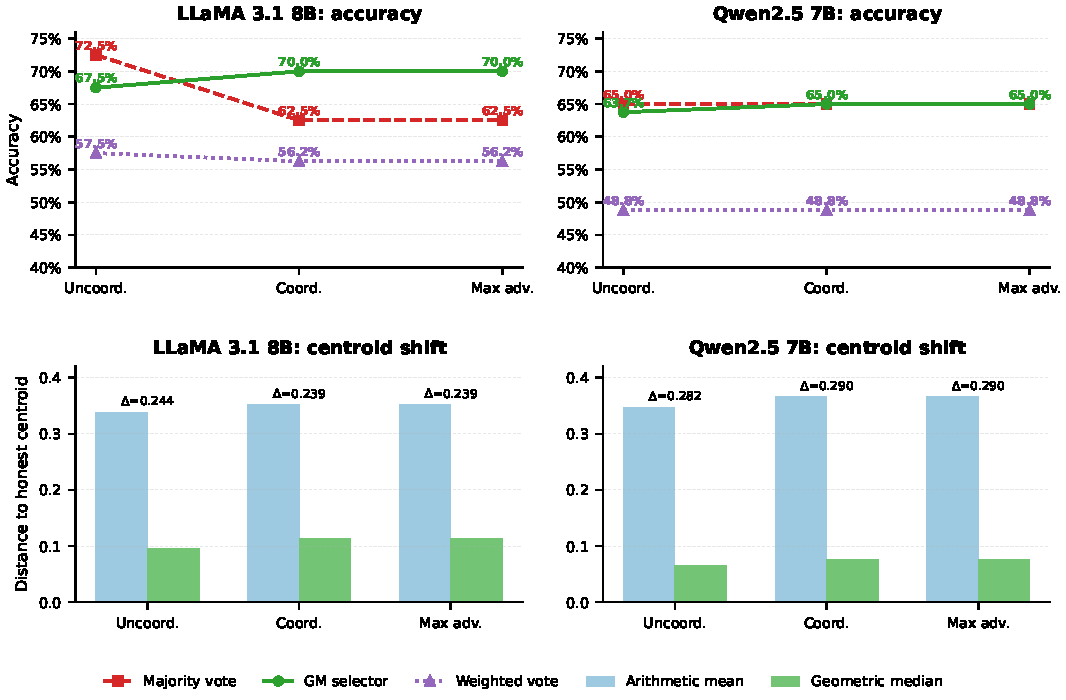
\includegraphics[width=\linewidth]{adversarial_coordination_acl}
\caption{Experiment~3: accuracy by coordination degree (top row) and centroid
  shift by coordination degree and model (bottom row).}
\label{fig:adversarial}
\end{figure*}

% ============================================================
\section{Multi-Provider Experiments}
\label{sec:multi}

\subsection{Experiment A: Provider Diversity}
\label{sec:exp-a}

To test whether multi-provider pools improve over the strongest single provider,
we constructed a mixed cache combining LLaMA 3.1 8B, Qwen2.5 7B, Mistral 7B
Instruct v0.3, and Phi-3 mini 4k in a 2-2-2-1 agent ratio ($N=7$ total) with
no fault injection. Per-provider $\tau$ calibration was applied.

\begin{table*}[t]
\centering
\caption{Experiment~A: multi-provider diversity results. \texttt{single\_X}
  conditions use $N=7$ agents from provider~X only.}
\label{tab:exp-a}
\small
\begin{tabular}{lccc}
\toprule
\textbf{Condition} & \textbf{Accuracy}
  & \textbf{Liveness Fallback Freq.} & \textbf{Mean Agents Admitted} \\
\midrule
\texttt{single\_llama}    & 0.6875 & 0.025 & 6.21 \\
\texttt{multi\_provider}  & 0.6750 & 0.038 & 6.05 \\
\texttt{single\_phi3}     & 0.6625 & 0.013 & 6.21 \\
\texttt{single\_qwen}     & 0.6625 & 0.088 & 6.56 \\
\texttt{single\_mistral}  & 0.5625 & 0.075 & 6.18 \\
\bottomrule
\end{tabular}
\end{table*}

The multi-provider pool does not outperform the strongest single provider:
\texttt{multi\_provider} achieves 67.5\% vs.\ \texttt{single\_llama} at 68.75\%
($-1.25$pp). This small difference should be interpreted cautiously, but it
indicates that provider diversity alone, without coordinated failures among wrong
agents, yields no observed accuracy advantage in this setup.

\subsection{Experiment B: Biased Provider Injection}
\label{sec:exp-b}

Experiment~B tests whether geometric median can tolerate a systematically biased
provider. Two designated biased providers (phi3, mistral) are evaluated under
natural bias (as-is generation) and injected bias (F1/F2 fault injection),
compared to an oracle condition (biased provider removed entirely).

\begin{table*}[t]
\centering
\caption{Experiment~B: biased provider results. \texttt{no\_X} = biased provider
  removed (oracle); \texttt{majority\_vote\_all} and \texttt{geometric\_median\_all}
  include all providers with majority vote or geometric median aggregation,
  respectively.}
\label{tab:exp-b}
\small
\begin{tabular}{lllc}
\toprule
\textbf{Biased Provider} & \textbf{Condition} & \textbf{Bias Type} & \textbf{Accuracy} \\
\midrule
\multirow{6}{*}{phi3}
  & \texttt{no\_phi3} (oracle)       & natural  & 0.675 \\
  & \texttt{majority\_vote\_all}     & natural  & \textbf{0.700} \\
  & \texttt{geometric\_median\_all}  & natural  & 0.675 \\
  & \texttt{no\_phi3} (oracle)       & injected & 0.675 \\
  & \texttt{majority\_vote\_all}     & injected & \textbf{0.725} \\
  & \texttt{geometric\_median\_all}  & injected & 0.675 \\
\midrule
\multirow{6}{*}{mistral}
  & \texttt{no\_mistral} (oracle)    & natural  & 0.700 \\
  & \texttt{majority\_vote\_all}     & natural  & \textbf{0.700} \\
  & \texttt{geometric\_median\_all}  & natural  & 0.675 \\
  & \texttt{no\_mistral} (oracle)    & injected & 0.700 \\
  & \texttt{majority\_vote\_all}     & injected & \textbf{0.7125} \\
  & \texttt{geometric\_median\_all}  & injected & 0.650 \\
\bottomrule
\end{tabular}
\end{table*}

Majority vote has higher observed accuracy than geometric median in every
condition. For Phi-3 injected bias, \texttt{majority\_vote\_all} reaches 0.725
while \texttt{geometric\_median\_all} remains at 0.675. For Mistral injected
bias, \texttt{geometric\_median\_all} degrades to 0.650 while
\texttt{majority\_vote\_all} reaches 0.7125.

\subsection{Mechanistic Interpretation}
\label{sec:multi-interp}

The contrast between Experiment~3 and Experiment~B is mechanistically
informative. In Experiment~3, 2 injected agents coordinate on the same wrong
answer, forming a tight cluster in embedding space. The 5 clean agents form a
larger cluster. Geometric median nearest-centroid improves LLaMA accuracy in
this setting.

In Experiment~B, a biased provider generates different wrong answers on different
questions (natural variation in model output). One or two diverse wrong votes
out of seven are usually handled by the honest majority. There is no tight
adversarial cluster for the geometric median to resist. Both majority vote and
geometric median are drawn toward the honest majority, and majority vote is
simpler and at least as accurate in this evaluation.

The relevant mechanism is cluster cohesion among wrong agents, not only the size
of the wrong minority. The centroid shift metric (Section~\ref{sec:centroid-shift})
quantifies this embedding-space effect: coordinated wrong answers form a tight
spatial cluster that the arithmetic mean is drawn toward more strongly than the
geometric median. Against scattered wrong answers, the observed advantage
disappears.

% ============================================================
\section{Discussion}
\label{sec:discussion}

\subsection{The Two-Failure-Mode Thesis}
\label{sec:thesis}

The experimental results support a unified thesis: the two structural failure
modes of self-consistency require distinct mechanisms, and no single pipeline
condition is optimal for both.

\begin{table*}[t]
\centering
\caption{Failure mode taxonomy and recommended conditions.}
\label{tab:failure-modes}
{\footnotesize
\setlength{\tabcolsep}{5pt}
\renewcommand{\arraystretch}{1.08}
\begin{tabularx}{\textwidth}{p{0.25\textwidth}p{0.28\textwidth}X}
\toprule
\textbf{Failure Mode}
  & \textbf{Highest observed condition}
  & \textbf{Mechanism} \\
\midrule
F1 crash / F3 drifter (invalid-format)
  & \texttt{hard\_only}; \texttt{soft\_weighting} strongest at $N=7$,
    $\beta=0.45$, F3-only
  & Module~1 drops low-confidence agents; liveness fallback matters
    when overloaded \\[6pt]
Experiment~1 F2 injection (spoofed logprob, invalid-format)
  & \texttt{hard\_only}
  & Spoofed agents pass Module~1; strict extraction and majority vote
    handles scattered wrong answers \\[6pt]
Coordinated valid-format attack (Exp~3)
  & \texttt{stage1\_only}
  & Strict extraction keeps adversarial votes; geometric median resists
    tight cluster \\[6pt]
Diverse provider bias (Exp~A/B)
  & majority vote
  & No tight cluster; geometric median offers no observed advantage \\
\bottomrule
\end{tabularx}
}
\end{table*}

Module~1 is effective when the broken agents fall far outside the clean TopKMass
cluster (F1 score$=0$, F3 score${\approx}2.3\times10^{-4}$). It is deliberately
ineffective against Experiment~1 F2 agents (TopKMass$=1.00$ by design), because
real logprob spoofing is a realistic threat in deployed systems and a filter that
is defeatable by logprob manipulation provides false assurance.

Module~2 (geometric median) is most useful when wrong agents form a spatially
coherent cluster in embedding space. Its robustness comes from minimizing the sum
of distances rather than squared distances. Squaring gives disproportionate
weight to outliers, so the arithmetic mean can be pulled far from the honest
majority by a coordinated wrong-answer cluster. By minimizing unsquared
distances, the geometric median limits this influence: a minority of fewer than
half the agents cannot move it arbitrarily far from the honest majority. The
centroid shift results ($+0.239$ to $+0.290$ embedding units, positive across
all conditions and both models) support this mechanism empirically, though
geometric proximity to the honest cluster does not guarantee that the
nearest-centroid agent's text matches the correct answer.

\subsection{Deprecated Aggregation Variants}
\label{sec:deprecated}

Two aggregation variants were explored before the final \texttt{stage1\_only}
framing.

The first variant is bidirectional NLI entailment verification, designed to check
whether the nearest-centroid candidate entails and is entailed by the
second-nearest agent's output. This path is retained in the repository for
provenance and helper reuse, but it is not the reported \texttt{full\_pipeline}
condition in Experiment~3.

The second variant is distance-weighted answer voting, the
\texttt{full\_pipeline} condition in the reported Experiment~3 results. It
underperforms \texttt{stage1\_only}
in every reported condition. Its main failure mode is vote fragmentation:
semantically diverse correct answers can split weighted vote mass, while a
coordinated wrong-answer cluster concentrates weight on one extractable answer.
Based on these results, the distance-weighted variant is not recommended;
TopKMass filtering combined with geometric median nearest-centroid is the
preferred configuration for the coordinated-attack setting.

\subsection{BFT Framing: Scope and Limitations}
\label{sec:bft}

The liveness threshold ($2f+1$ with $f = \lfloor(N-1)/3\rfloor$) and fault
fraction vocabulary ($\beta$) are drawn from Byzantine Fault Tolerance theory.
This framing is useful for reasoning about worst-case degradation scenarios and
for specifying the pipeline's behavior when the fault load exceeds design
thresholds. It should not be interpreted as a claim that the system provides
Byzantine-fault-tolerant consensus in the classical sense.

The current evaluation uses a homogeneous pool ($N$ samples from one model). In
this setting, no agent has an incentive to deceive; the Experiment~1 F2
construction and the Experiment~3 coordinated attack are synthetic stress tests,
not real-world threats. The BFT framing becomes more
motivated in a multi-provider heterogeneous setting, where a provider operating
one or more agents may have incentives to steer the consensus answer. The
coordinated-attack defense is a hypothesis for coordinated provider failures, not
a result established by the natural provider-bias experiments here.

\subsection{Limitations}
\label{sec:limitations}

\paragraph{Small evaluation set and aggregate CSVs.}
Each main evaluation uses 80 questions per model after the 20\% dev split, so
absolute accuracy values carry non-trivial uncertainty. The canonical Experiment~1
and Experiment~3 CSVs store aggregate accuracies rather than per-question
correctness vectors; reporting paired confidence intervals would require
re-extracting question-level outcomes from the generation caches. We therefore
interpret small differences cautiously.

\paragraph{Qwen calibration artifact.}
Qwen's 13.75\% liveness fallback rate at $\beta=0$ and 11.25\% in Experiment~3
indicate that the 5th-percentile $\tau$ over-filters Qwen clean agents. This
reduces Module~1's effective contribution for Qwen and explains the neutral
Experiment~3 result. Adaptive per-model calibration with larger dev slices would
likely improve Qwen's results.

\paragraph{Homogeneous pool.}
All primary experiments use $N=7$ samples from a single model at
temperature$=0.7$. Diversity within the pool is stochastic, not structural. The
multi-provider experiments (Section~\ref{sec:multi}) extend to four models but
find neutral or negative results for multi-provider consensus under
non-coordinated conditions.

\paragraph{Synthetic fault injection.}
Experiment~1 F2 agents use a fixed invalid-format template with perfectly
spoofed logprobs, whereas Experiment~3 separately uses valid-format coordinated
wrong answers. Real-world failure modes may have different logprob signatures or
different patterns of answer coordination. The centroid shift metric provides
mechanistic evidence about embedding-space behavior, but accuracy results may
differ under different adversarial strategies.

\paragraph{Embedding-model dependency.}
All Module~2 results use a single sentence encoder
(\texttt{sentence-transformers/all-mpnet-base-v2}, 768-dimensional). The
geometric-median selector's behavior depends on the encoder's geometry, and
results may shift under different encoders (alternative MTEB tiers,
domain-tuned encoders, or contrastive vs.\ instruction-tuned objectives). We
do not report encoder-sensitivity ablations and treat the encoder as a fixed
component of the evaluated system.

\paragraph{Task and language scope.}
The evaluation uses two English datasets, GSM8K (arithmetic reasoning) and
StrategyQA (multi-hop commonsense). Findings about strict extraction,
TopKMass, and geometric-median nearest-centroid are not assumed to transfer to
other task types (open-ended generation, code synthesis, dialog) or to
non-English inputs without further evaluation.

% ============================================================
\section{Conclusion}
\label{sec:conclusion}

We have presented a failure-mode-specific study of multi-agent LLM consensus
under two structurally distinct failure modes of self-consistency. Strict answer
extraction prevents invalid outputs from being counted as votes by abstaining
when no parseable answer is found. TopKMass filtering identifies low-confidence
invalid-format outputs using a stable-region sliding-window mean of top-5 token
probabilities. Geometric median nearest-centroid aggregation provides a separate
mechanism for coordinated valid-format wrong answers by minimizing sum of
embedding distances rather than sum of squared distances.

The primary Experiment~1 result is methodological: strict answer extraction, a
correction to baseline self-consistency rather than a new consensus mechanism,
removes a 16.5 percentage point accuracy collapse in LLaMA majority-vote
results at high fault fractions. At $\beta=45\%$, the all-fault aggregate
favors TopKMass filtering plus strict majority vote over the strict-extraction
baseline (LLaMA 0.727 vs.\ 0.708; Qwen 0.656 vs.\ 0.648). Experiment~2 validates TopKMass as the strongest of the tested
logprob-based correctness predictors (AUC$=0.612$ for LLaMA, vs.\ 0.580 for
negated entropy and 0.448 for negated logprob variance), while confirming that
its primary value is detecting broken agents far outside the clean cluster rather
than discriminating correct from incorrect among healthy agents. Experiment~3
shows that geometric median nearest-centroid improves LLaMA accuracy by 7.5pp
over majority vote under coordinated synthetic wrong-answer injection.
Multi-provider experiments delineate the scope of this defense: it requires
coordinated wrong answers forming a tight cluster and does not extend to natural
provider diversity or scattered provider bias in this evaluation.

No single pipeline condition is uniformly optimal. Strict extraction and TopKMass
filtering are most useful for invalid-format failures; geometric median
nearest-centroid is most useful when wrong answers form a coordinated semantic
cluster; majority vote remains simpler and at least as effective in several
uncoordinated regimes. Understanding the specific conditions under which each
mechanism helps, supported by mechanistic metrics such as TopKMass AUC and
centroid shift, is the primary contribution of this work.

Future directions include: (1) multi-provider heterogeneous pools with mixed
logprob availability, including providers that do not expose per-token logprobs;
(2) adaptive $\tau$ calibration per provider or per output length using larger
dev slices; (3) larger evaluation sets with per-question confidence intervals;
(4) arithmetic-mean nearest-centroid and other additional aggregation ablations;
and (5) streaming consensus settings where agent count varies dynamically.

% ============================================================
\FloatBarrier
\bibliographystyle{acl_natbib}
\bibliography{references}
\clearpage

% ============================================================
\appendix

\section{Additional Figures and Tables}
\label{app:figures}
\FloatBarrier

\begin{figure}[!t]
\centering
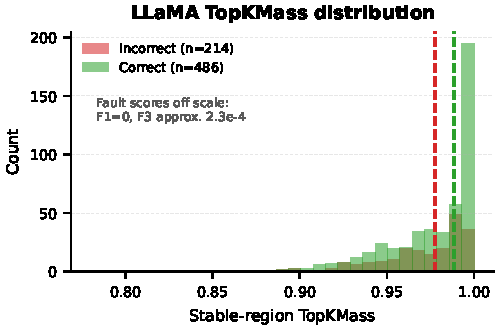
\includegraphics[width=\columnwidth]{topkmass_distribution_acl}
\caption{Histogram of TopKMass score distributions for correct vs.\ incorrect
  clean agents (LLaMA 3.1 8B, 700 agents, no faults injected). Dashed vertical
  lines mark class medians. Fault-agent scores (F1: 0.0,
  F3: ${\approx}2.3\times10^{-4}$) are far off-scale to the left and not shown.}
\label{fig:topkmass-dist}
\end{figure}

\begin{figure*}[!t]
\centering
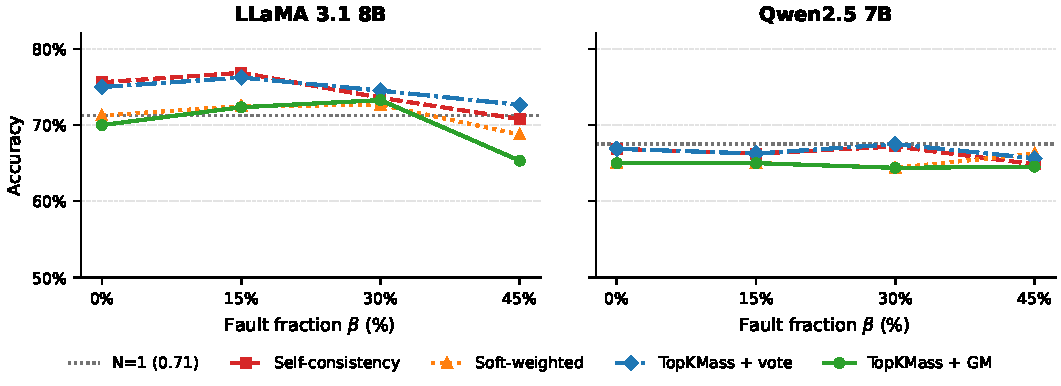
\includegraphics[width=\linewidth]{accuracy_vs_beta_acl}
\caption{Experiment~1: accuracy vs.\ fault fraction $\beta$ including the $N=1$
  single-agent reference line (gray dotted). The $N=1$ reference is flat by
  construction: $\lfloor 1 \times \beta \rfloor = 0$ for any
  $\beta \in \{0,\,0.15,\,0.30,\,0.45\}$, so the single agent's generation is
  never perturbed by fault injection. This line should be read as an unperturbed
  single-agent accuracy floor, not as a condition exposed to the same fault rate
  as the ensemble conditions.}
\label{fig:accuracy-beta-n1}
\end{figure*}

\begin{figure*}[!t]
\centering
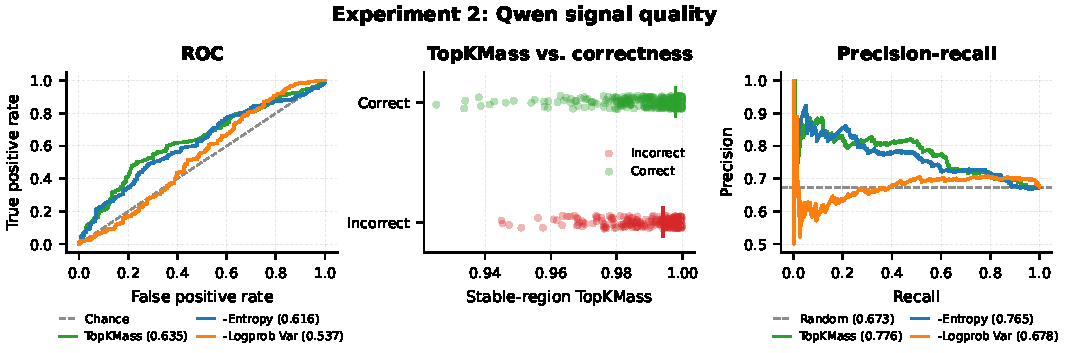
\includegraphics[width=\linewidth]{experiment_2_signals_qwen_acl}
\caption{Experiment~2 (Qwen2.5 7B): signal quality panels, parallel to
  Figure~\ref{fig:signals} in the main body. Qwen TopKMass AUC (0.635) exceeds
  LLaMA (0.612); negated entropy is a closer second for Qwen (AUC gap 0.019
  vs.\ 0.032 for LLaMA). Logprob variance remains weak for Qwen
  (AUC$=0.538$, though above the LLaMA value of 0.448). The narrower TopKMass
  score range for Qwen ($[0.97,\,1.00]$, 5th percentile to max) vs.\ LLaMA
  ($[0.91,\,1.00]$, with a lower tail to approximately 0.72) reflects Qwen's
  generally higher per-token confidence and contributes to the calibration
  artifact observed in Experiments~1 and~3.}
\label{fig:qwen-signals}
\end{figure*}

\begin{table*}[!t]
\centering
\caption{Liveness fallback frequency by condition, $N$, $\beta$, and model,
  averaged over the four fault types (F1, F2, F3, mix) in
  \texttt{experiment\_1\_\{llama,qwen\}\_v4.csv}. At $\beta=0.45$ with $N=7$,
  $\lfloor 7 \times 0.45 \rfloor = 3$ faults; the BFT liveness threshold is
  $2f+1=5$ admitted agents. F1-only and F3-only slices individually trigger
  fallback at 100\% of questions in this regime, while F2 retains all
  spoofed-pass agents at 0\% fallback, so the all-fault average falls between
  these extremes.}
\label{tab:liveness}
\small
\begin{tabular}{llccccc}
\toprule
\textbf{Model} & \textbf{Condition} & \textbf{N}
  & $\bm{\beta}=0$\% & $\bm{\beta}=15$\%
  & $\bm{\beta}=30$\% & $\bm{\beta}=45$\% \\
\midrule
LLaMA 3.1 8B & \texttt{hard\_only}   & 7 & 5.00\%  & 5.94\%  & 11.25\% & 53.13\% \\
LLaMA 3.1 8B & \texttt{full\_system} & 7 & 5.00\%  & 5.94\%  & 11.25\% & 53.13\% \\
Qwen2.5 7B   & \texttt{hard\_only}   & 7 & 13.75\% & 16.56\% & 20.00\% & 57.81\% \\
Qwen2.5 7B   & \texttt{full\_system} & 7 & 13.75\% & 16.56\% & 20.00\% & 57.81\% \\
\bottomrule
\end{tabular}
\end{table*}

\texttt{hard\_only} reduces to the unfiltered baseline under F1/F3 at
$\beta=0.45$, $N=7$, since fallback admits the full pool at 100\% of questions
when 3 of 7 agents are filtered and the remaining 4 are below the $2f+1=5$
threshold. \texttt{full\_system} does not strictly reduce to baseline in this
regime: even when the liveness flag is set, geometric median nearest-centroid
still selects from the admitted (possibly degraded) pool rather than performing
strict majority voting, which produces different answers on a subset of
questions. Empirically, for $N=7$, $\beta=0.45$, F1: LLaMA \texttt{baseline}
$=$ \texttt{hard\_only} $= 0.7375$ but \texttt{full\_system} $= 0.6375$; Qwen
\texttt{baseline} $=$ \texttt{hard\_only} $= 0.675$ but \texttt{full\_system}
$= 0.6625$. For F3, Qwen \texttt{baseline} $=$ \texttt{hard\_only} $= 0.575$
while \texttt{full\_system} $= 0.6375$. The remaining differences between
conditions in Table~\ref{tab:exp1-results} at $\beta=0.45$ are jointly driven
by this fallback-time selector behavior and by Experiment~1 F2 questions, where
spoofed logprobs pass Module~1 and filtering remains active.

\section{Reproducibility: Code Paths and Result Artifacts}
\label{app:code}

The canonical TopKMass filter is implemented in \texttt{pipeline/filter.py}. The
final geometric median nearest-centroid helper is implemented in
\texttt{pipeline/stage1.py}, reusing embedding and geometric-median helpers from
\texttt{pipeline/aggregation.py}. The older NLI verification path remains in
\texttt{pipeline/aggregation.py} for provenance and helper reuse. The
distance-weighted voting ablation used by the Experiment~3 \texttt{full\_pipeline}
rows is implemented in \texttt{pipeline\_v2/aggregation.py}.

The main runners are \texttt{eval/runner\_v2.py},
\texttt{eval/signal\_quality.py}, and \texttt{eval/adversarial\_test\_v2.py}.
Multi-provider experiments use \texttt{eval/runner\_multi.py},
\texttt{eval/biased\_provider\_test.py}, and \texttt{pipeline\_multi/}; shared
I/O helpers are in \texttt{eval/io.py} and \texttt{eval/answer\_extraction.py}.

The main result artifacts are \texttt{results/experiment\_1\_llama\_v4.csv},
\texttt{results/experiment\_1\_qwen\_v4.csv}, the Experiment~2 signal-quality
directories under \texttt{results/exp2\_*}, the Experiment~3 \texttt{\_v2.csv}
files under \texttt{results/exp3\_*}, and the multi-provider CSVs in
Section~\ref{sec:multi}. Confidence intervals are omitted because the canonical
Experiment~1 and Experiment~3 CSVs contain aggregate accuracies rather than
per-question correctness vectors.

\end{document}
